%%%%%%%%%%%%%%%%%%%%%%%%%%%%%%%%%%%%%%%%%
% baposter Portrait Poster
% LaTeX Template
% Version 1.0 (15/5/13)
%
% Created by:
% Brian Amberg (baposter@brian-amberg.de)
%
% This template has been downloaded from:
% http://www.LaTeXTemplates.com
%
% License:
% CC BY-NC-SA 3.0 (http://creativecommons.org/licenses/by-nc-sa/3.0/)
%
%%%%%%%%%%%%%%%%%%%%%%%%%%%%%%%%%%%%%%%%%

%----------------------------------------------------------------------------
%	PACKAGES AND OTHER DOCUMENT CONFIGURATIONS
%----------------------------------------------------------------------------

\documentclass[a0paper,landscape,fontscale=0.395]{baposter}

\usepackage[font=small,labelfont=bf]{caption} % Required for specifying captions to tables and figures
\usepackage{booktabs} % Horizontal rules in tables
\usepackage{enumitem} % To change spacing in itemize and enumerate lists
\usepackage{multicol}
\usepackage{relsize} % Used for making text smaller in some places
\usepackage{amsfonts, amsmath, amsthm, amssymb} % For math fonts, symbols and environments
\usepackage{wrapfig} % Allows wrapping text around tables and figures
\usepackage[export]{adjustbox}% http://ctan.org/pkg/adjustbox
\usepackage{palatino} % Uncomment to use the Palatino font
\usepackage{graphicx} % Required for including images
\usepackage{graphbox}
\usepackage{color}
\usepackage{mathtools}
\usepackage{hyperref}

\graphicspath{{figures/}} % Directory in which figures are stored

\definecolor{bordercol}{RGB}{256,256,256} % Border color of content boxes
\definecolor{headercol1}{RGB}{51,0,111} % Background color for the header in the content boxes (left side)
\definecolor{headercol2}{RGB}{51,0,111} % Background color for the header in the content boxes (middle)
\definecolor{headerfontcol}{RGB}{256,256,256} % Text color for the header text in the content boxes
\definecolor{boxcolor}{RGB}{256,256,256} % Background color for the content in the content boxes

\newenvironment{Figure}
  {\par\medskip\noindent\minipage{\linewidth}}
  {\endminipage\par\medskip}

\DeclarePairedDelimiterX{\norm}[1]{\lVert}{\rVert}{#1}
\DeclareMathOperator{\Tr}{Tr}

\begin{document}

\begin{poster}{
    columns=3,
    grid=false,
    headerheight=0.1\textheight,
    borderColor=bordercol, % Border color of content boxes
    headerColorOne=headercol1, % Background color for the header in the content boxes (left side)
    headerColorTwo=headercol2, % Background color for the header in the content boxes (middle)
    headerFontColor=headerfontcol, % Text color for the header text in the content boxes
    boxColorOne=boxcolor, % Background color for the content in the content boxes
    headershape=roundedright, % Specify the rounded corner in the content box headers
    headerfont=\Large\sf\bf, % Font modifiers for the text in the content box headers
    textborder=rectangle,
    background=none,
    headerborder=open, % Change to closed for a line under the content box headers
    boxshade=plain
}
{}
%
%----------------------------------------------------------------------------
%	TITLE AND AUTHOR NAME
%----------------------------------------------------------------------------
%
{\sf\bf Deep learning for analysis of diffusion-MRI based white matter tractometry} % Poster title
{%
    \vspace{1em}
    Joanna Qiao{$^1$}, Jason Yeatman{$^2$}, Ariel Rokem{$^1$}, Adam Richie-Halford{$^2$}
    \\ Contact: arokem@uw.edu, adamrh@stanford.edu \hspace{0.5em} \null \\ % Author names (cont)
    {\smaller%
        1. University of Washington, %
        2. Stanford University %
        \hfill %
    }
} % Author affiliations and email addresses
{%

\includegraphics[align=c,height=3.00cm]{logos/UWlogo.png}%

\includegraphics[align=c,height=3.20cm]{logos/stanford_logo.png}%
} % University/lab logos
\vspace{-10em}

%----------------------------------------------------------------------------
%	INTRODUCTION
%----------------------------------------------------------------------------

\headerbox{Introduction}{name=introduction, column=0, row=0}{

\begin{itemize}[nosep, leftmargin=*]
    \item Tractometry uses diffusion MRI (dMRI) to quantify brain tissue properties within white matter connections \emph{in vivo} \cite{yeatman2012}.
    \item The Healthy Brain Network Processed Open Derivatives (HBN POD2) is a
    large (n>2,000) pediatric dMRI dataset that has been processed and automatically QC'd\cite{RichieHalfordCieslak2022HBNPOD2, alexander2017hbn}.
    \item The pyAFQ software was used to create tract profiles for statistical analysis \cite{Kruper2021evaluating}.
    \item In previous work, we demonstrated that regularized regression provides accurate predictions of individual age in HBN from tractometry data (WM-based ``brain age'')\cite{richford2021sgl}.
\end{itemize}

\vspace{0.5em}
\noindent\textbf{%
    \underline{Question}: %
    Would convolutional neural networks provide improvements in inferences from tractometry?%
}
\vspace{0.5em}}

\headerbox{Methods}{name=methods, column=0, below=introduction}{
\begin{itemize}[nosep, leftmargin=*]
\end{itemize}


\begin{minipage}[b]{1\linewidth}
    \large
    \begin{minipage}[b]{0.35\linewidth}
    \textbf{A}\\
    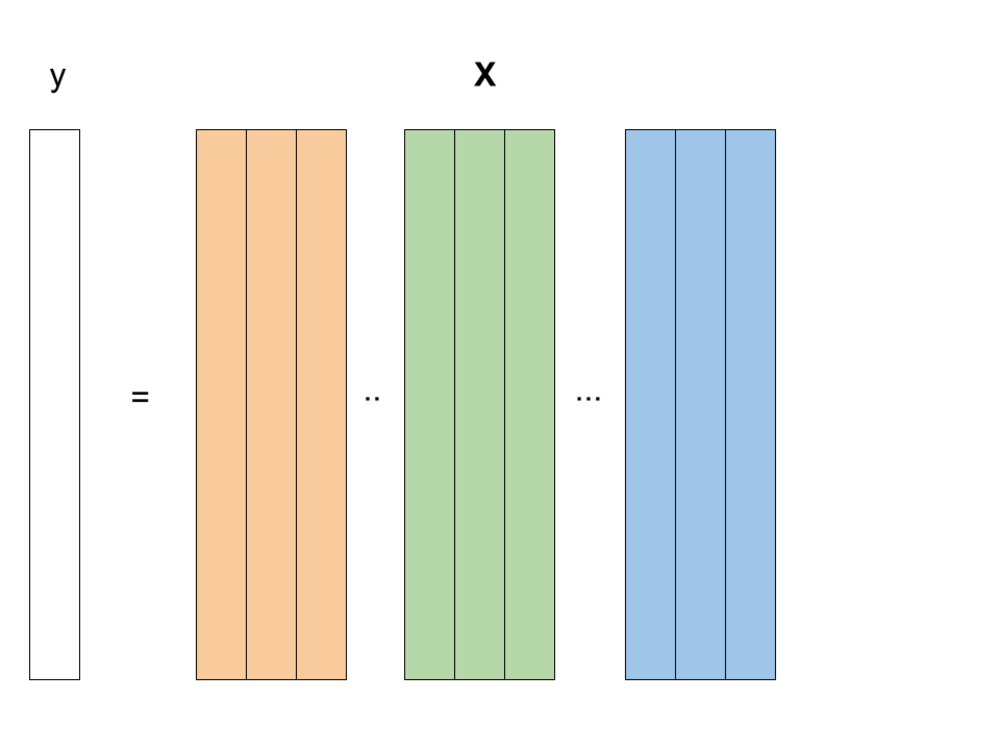
\includegraphics[height=4.5cm]{figures/linear-model.pdf}
    \end{minipage}
    \hspace{0.5cm}
    \begin{minipage}[b]{0.35\linewidth}
    \textbf{B}\\
    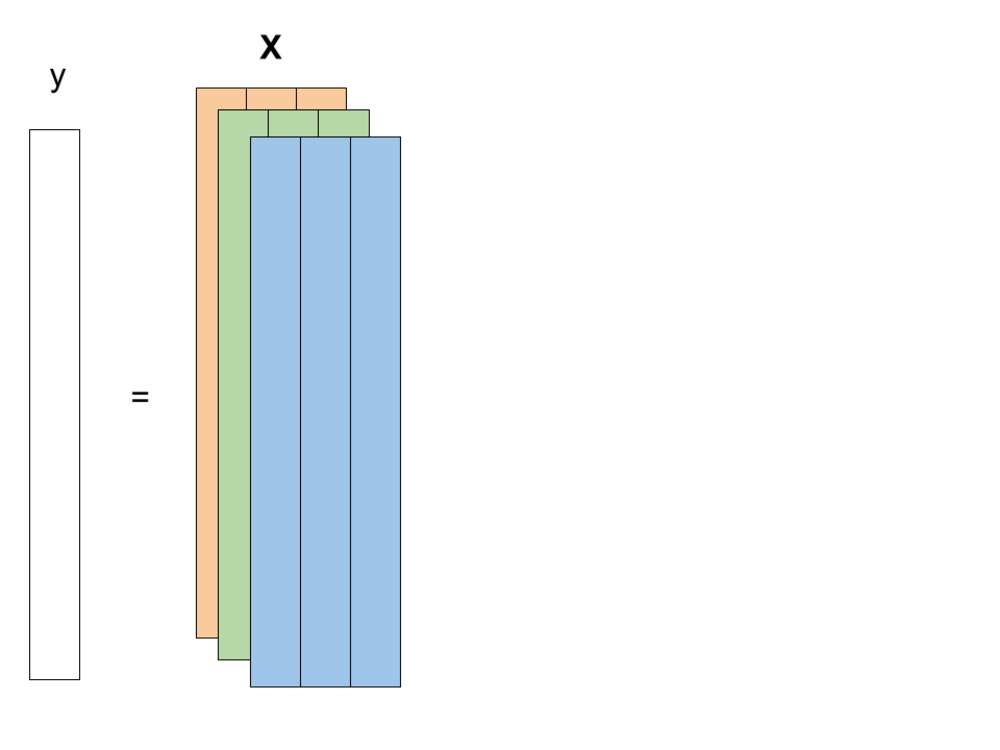
\includegraphics[height=4.5cm]{figures/linear-to-convnet.pdf}
    \end{minipage}
    \begin{minipage}[b]{0.2\linewidth}
    \textbf{C}\\
    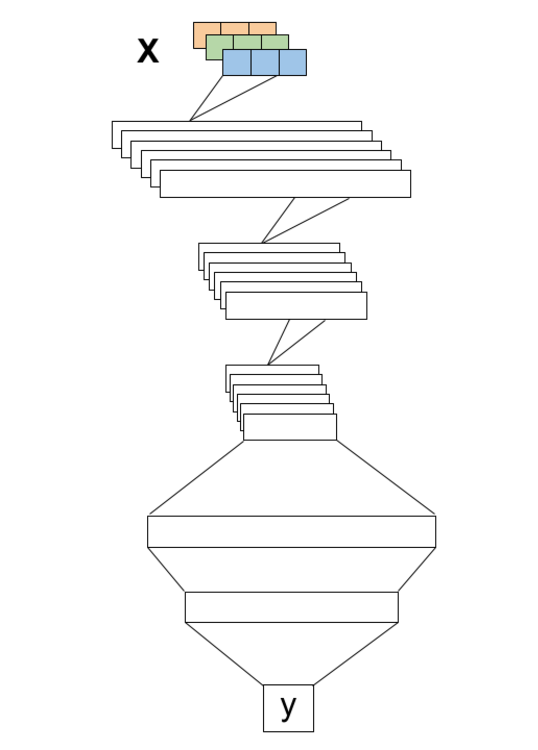
\includegraphics[height=4.5cm]{figures/convnet-schematic.pdf}
    \end{minipage}
 \end{minipage}

In a linear tractometry model, $\textbf{y} = \beta X$ (\textbf{A}), to move towards a convolutional neural networks, we stack the data from different tracts and metrics (FA, MD, MK) as different measurement ``channels'' (\textbf{B}). Training samples are then passed to a network (\textbf{C}).

We used the 1817 subjects from HBN POD2 that had passing QC scores and age
information.

To evaluate the models, we set aside a test set of 20\% of the subjects (363 subjects)

To compare model dependence on training set size, we set aside a test set (20\% or ) and then trained with variable train set sizes (100, 175, 350, 700, 1000, 1453 subjects)
}

%----------------------------------------------------------------------------
%	RESULTS 1
%----------------------------------------------------------------------------

\headerbox{Results}{name=results, column=1, span=2, row=0}{

\begin{multicols}{3}
    \begin{Figure}
        \centering
        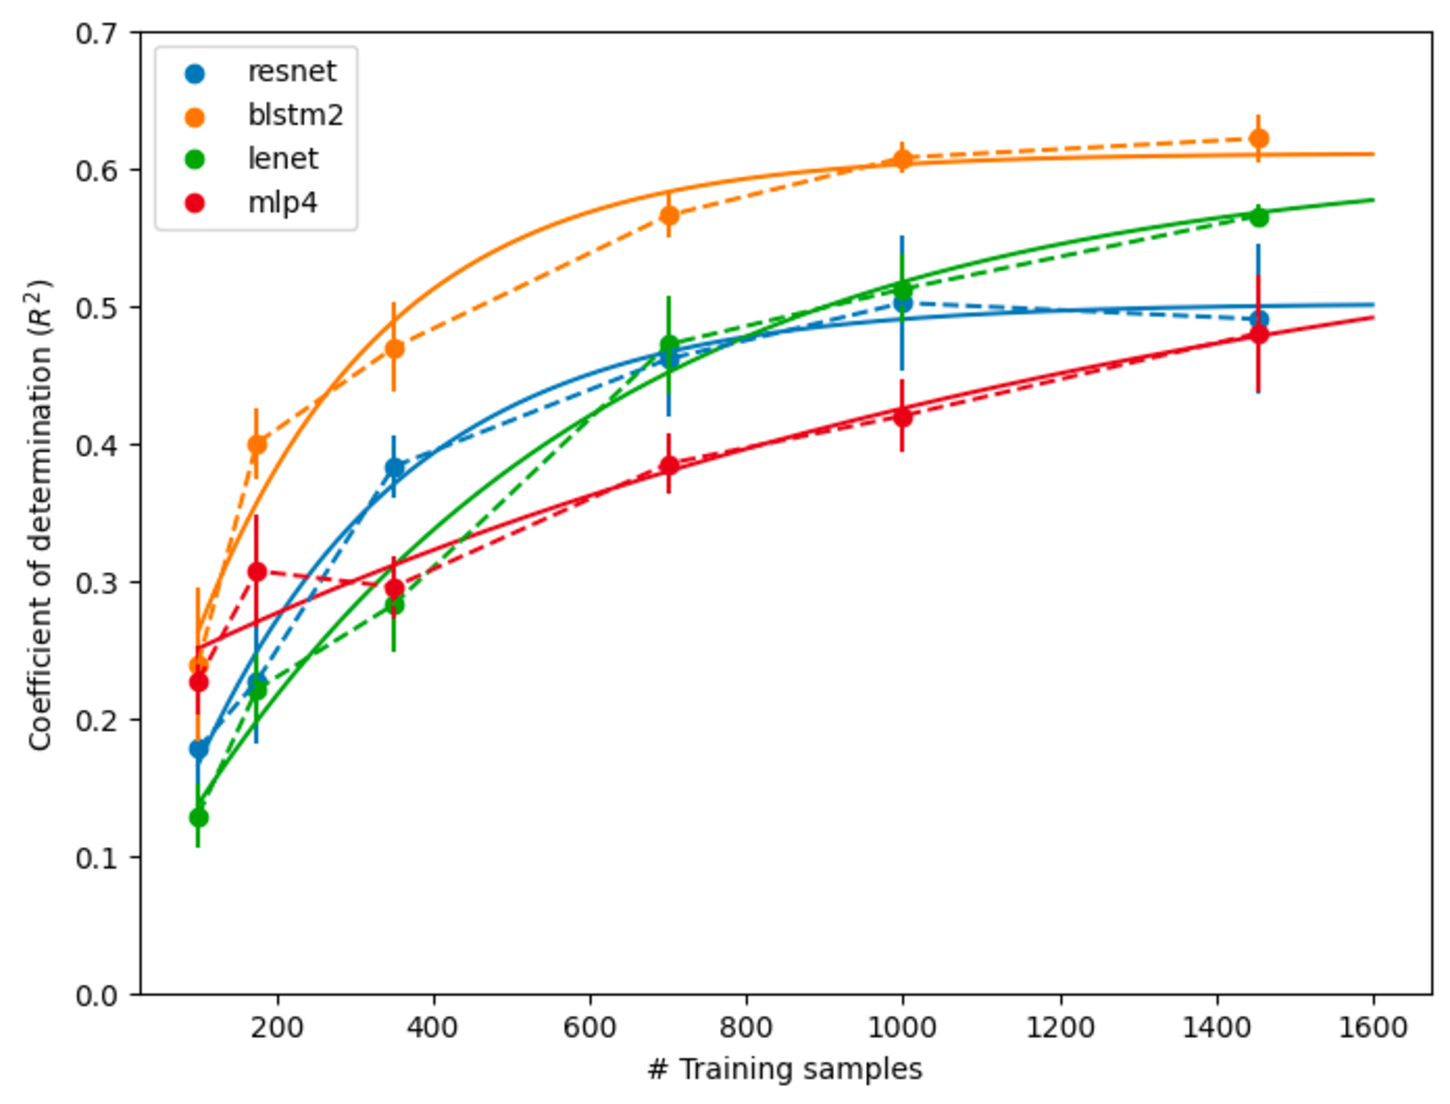
\includegraphics[width=0.33\linewidth]{figures/results_no_aug}
        \captionof{figure}{
            {\bf XXX}:
           XXX
        }
    \end{Figure}
    \columnbreak
    \begin{Figure}
        \centering
        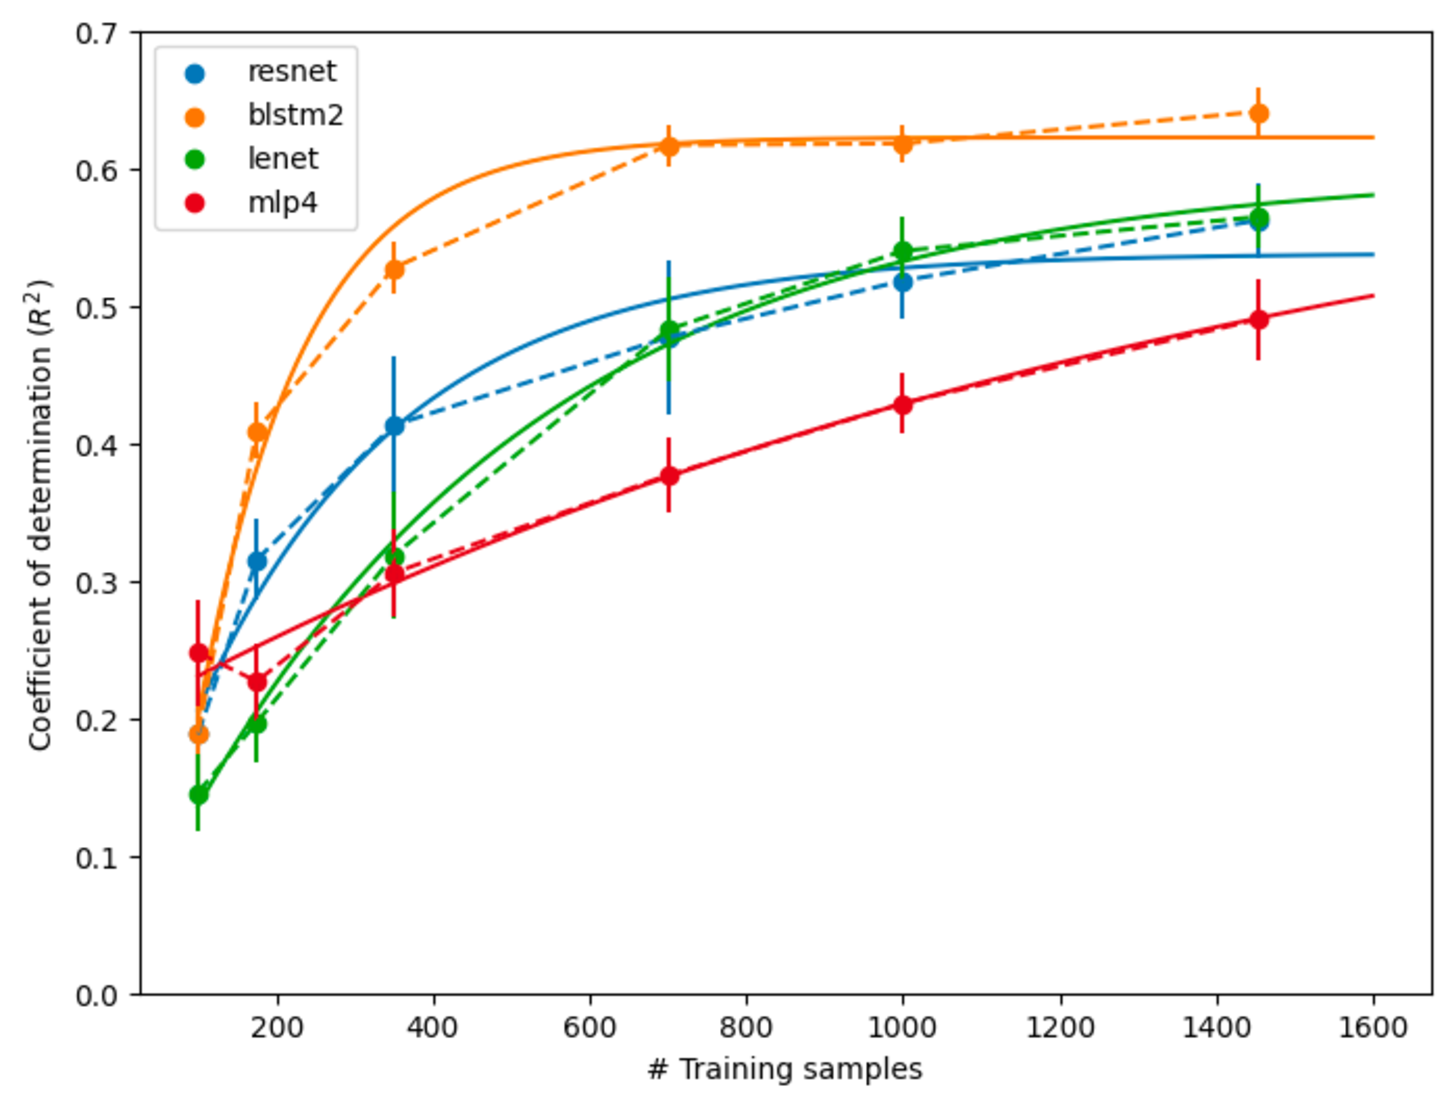
\includegraphics[width=0.33\linewidth]{figures/results_low_aug.pdf}
        \captionof{figure}{
            {\bf XXX}:
            XXX
            }
    \end{Figure}

    \columnbreak
    \begin{Figure}
        \centering
        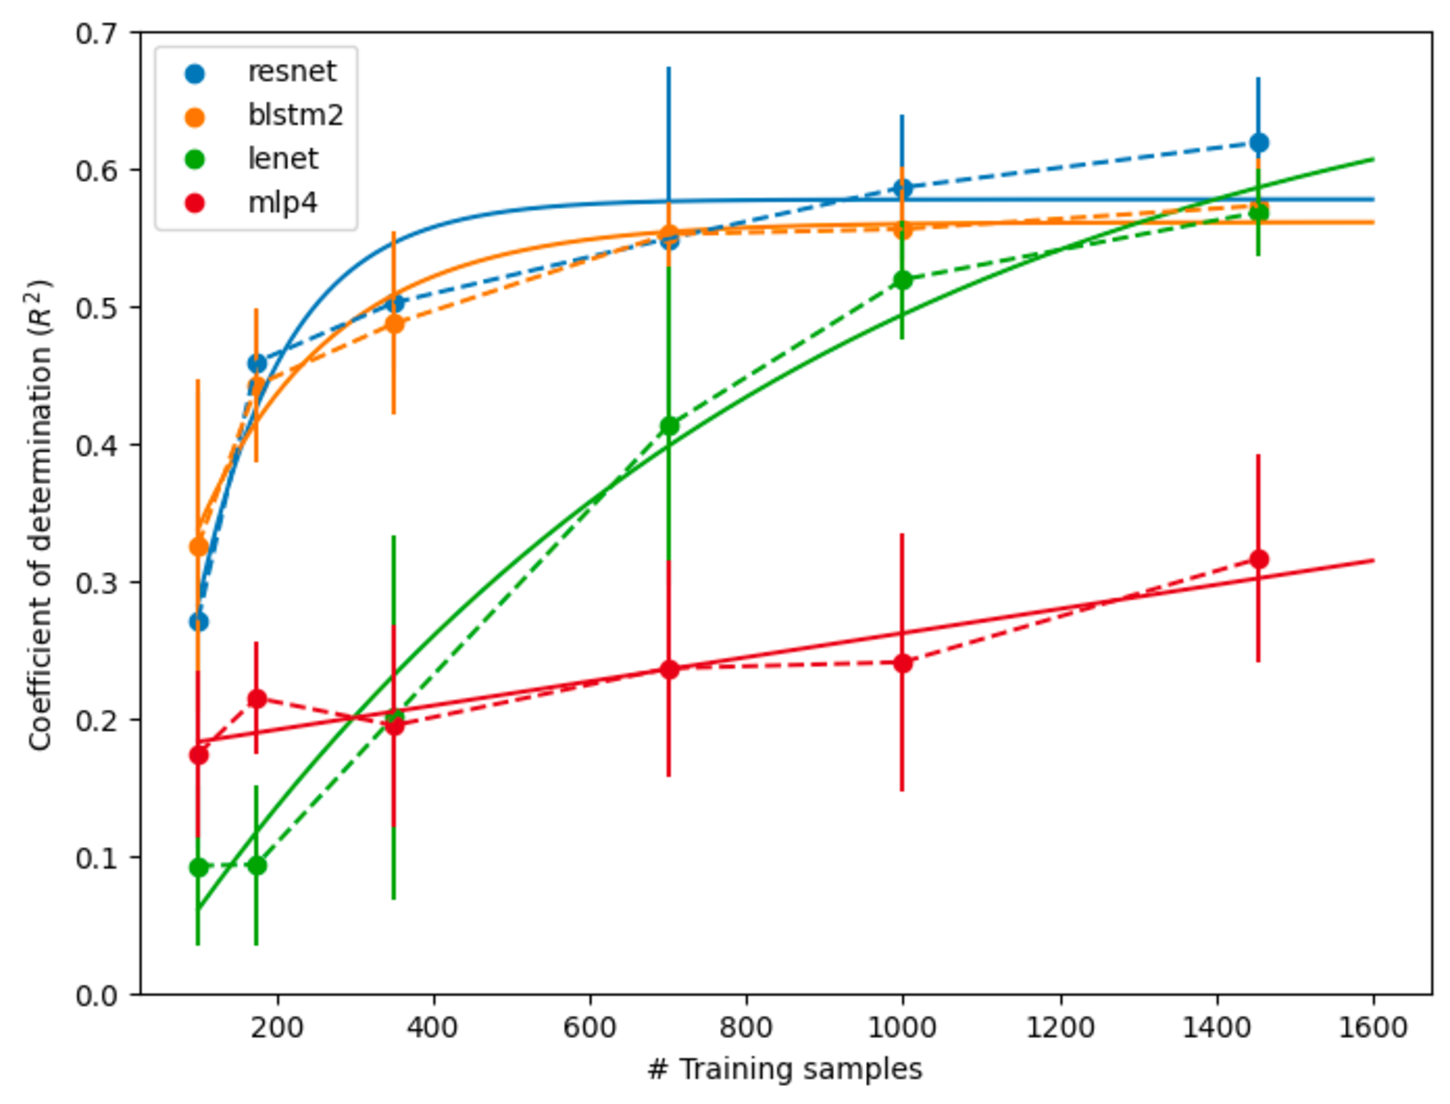
\includegraphics[width=0.33\linewidth]{figures/results_high_aug.pdf}
        \captionof{figure}{
            {\bf XXX}:
            XXX
        }
    \end{Figure}

    \vspace{2em}
\end{multicols}

}

%----------------------------------------------------------------------------
%	CONCLUSION
%----------------------------------------------------------------------------

\headerbox{Conclusion and future work}{name=conclusion, column=2, below=methods}{

XXX

}

%----------------------------------------------------------------------------
%   REFERENCES
%----------------------------------------------------------------------------

\headerbox{References}{name=references,column=0,span=2,below=conclusion,above=bottom}{

\begin{multicols}{2}
\smaller \smaller % Reduce the font size in this block
\renewcommand{\section}[2]{\vskip 0.05em} % Get rid of the default "References" section title
\nocite{*} % Insert publications even if they are not cited in the poster

% \printbibliography
\bibliographystyle{unsrt}
\bibliography{poster}
\end{multicols}
}

%----------------------------------------------------------------------------
%	ACKNOWLEDGMENTS
%----------------------------------------------------------------------------

\headerbox{Acknowledgments}{name=acknowledgments, column=2, below=conclusion,above=bottom}{

\begin{multicols}{2}
\smaller % Reduce the font size in this block

\includegraphics[height=1.0cm]{logos/nimh-logo.png}


\includegraphics[height=0.75cm]{logos/eSciencelogo.png}

\end{multicols}
}

\end{poster}

\end{document}
